\documentclass{beamer}
%\usepackage{forloop}
\usepackage{color,tikz}
\usepackage{hyperref}
\hypersetup{colorlinks=true, linkcolor=black, citecolor=black, urlcolor=blue}

\usepackage[
  backend=bibtex,
  style=numeric-comp,sorting=none,block=ragged,firstinits=false
]{biblatex}
\bibliography{tilelvreqs}

\definecolor{class}{RGB}{111,159,207}
\definecolor{literal}{rgb}{0.58,0,0.82}

\let\Tiny=\tiny

\setbeamersize{text margin left=20px,text margin right=20px}
\setbeamertemplate{navigation symbols}{}
\setbeamertemplate{section in toc}[sections numbered]
\setbeamertemplate{subsubsection in toc}[subsubsections numbered]
\setbeamertemplate{footline}{%
  \usebeamerfont{author in head/foot}%
  \insertshortauthor[width={1.7cm},respectlinebreaks,center]%
  \hspace*{-0.8mm},\ %
  \usebeamerfont{date in head/foot}\insertdate%
  \hspace*{1mm}%
  \usebeamerfont{footline}\url{https://indico.cern.ch/event/467725/}%
  \hfill%
  \insertframenumber/\inserttotalframenumber%
  \hspace*{1mm}
}
\setbeamertemplate{bibliography item}{\insertbiblabel}

\def\changemargin#1#2{\list{}{\rightmargin#2\leftmargin#1}\item[]}
\let\endchangemargin=\endlist

\title{Low Voltage Monitoring Upgrade\\for ATLAS Tile Calorimeter}
\author[Ivan Pogrebnyak]
{%
  \texorpdfstring{
    \centering
    I. Pogrebnyak \\
    Working with: A. Paramonov, G. Drake, J. Proudfoot \\
  }{Ivan Pogrebnyak}
}
\date{December 8, 2015}

\begin{document}

\frame{
  \begin{tikzpicture}[remember picture,overlay]
    \node[anchor=north west] at (current page.north west){
      
\includegraphics[height=30pt]{logos/msu_helmet}
      \vspace{5px}
      
\includegraphics[height=30pt]{logos/msu_text}
    };
    \node[anchor=north east] at (current page.north east){
      \begin{minipage}{100px}
      \vspace{-21px}
      {\huge Argonne}\\
      {\large National Laboratory}
      \end{minipage}
      
\includegraphics[height=30pt]{logos/argonne_logo}
    };
    \node[anchor=south west] at (current page.south west){
      \begin{minipage}{100px}
      
\includegraphics[height=30pt]{logos/DOE_Logo_Color}
      \vspace{8px}
      \end{minipage}
    };
    \node[anchor=south east] at (current page.south east){
      \begin{minipage}{96px}
      {\huge ATLAS}
      \vspace{-21px}\\
      {\large Experiment}
      \hspace{5px}
      
\includegraphics[height=30pt]{logos/cern_logo}
      \vspace{8px}
      \end{minipage}
    };
  \end{tikzpicture}

  %\vspace{20px}
  \titlepage
}

\frame{\frametitle{Table of contents}
  \tableofcontents
}

\section{foog bar}

\frame{\frametitle{TileCal electronics (at a glance)}
  \begin{changemargin}{-20px}{-20px}
    \centering
    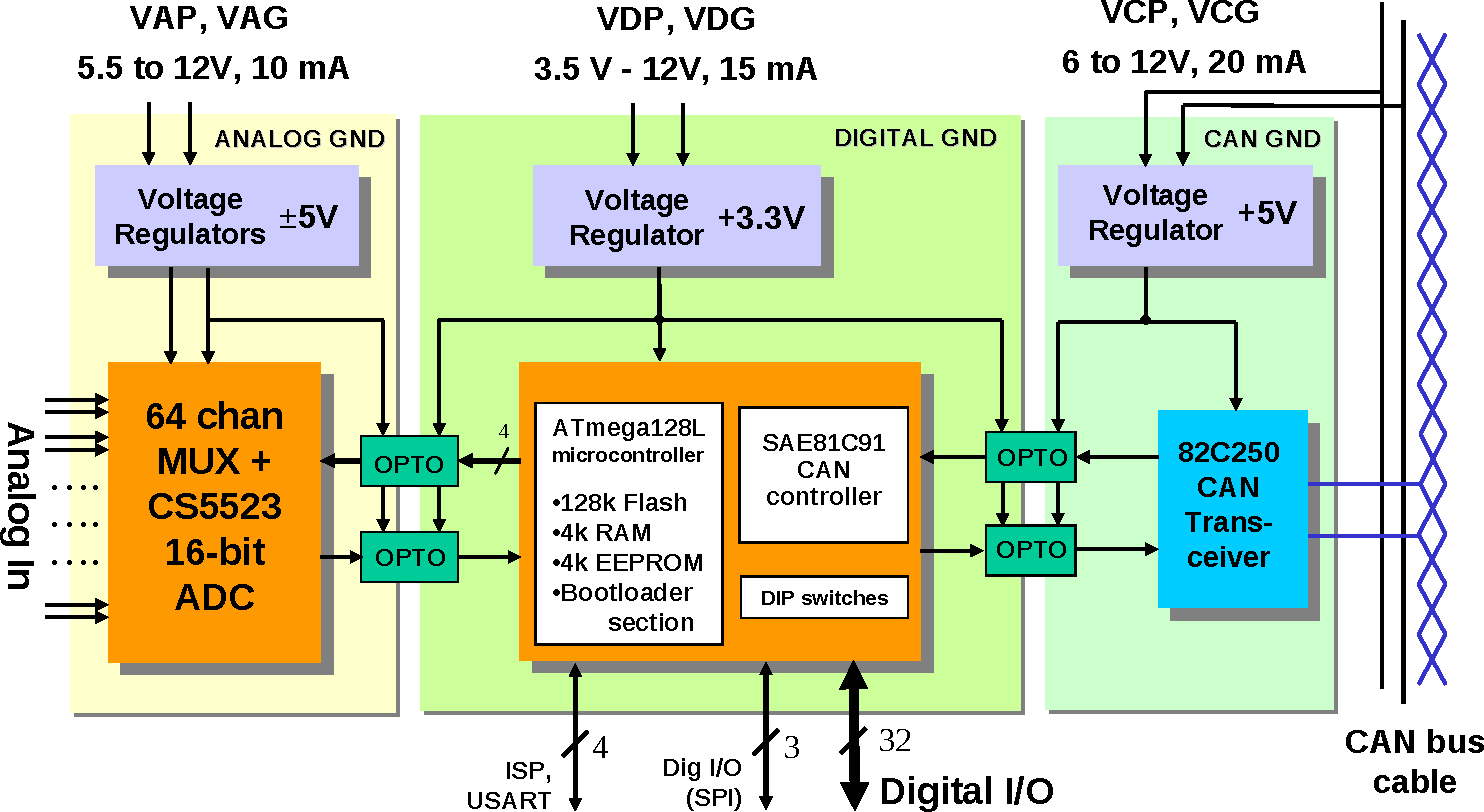
\includegraphics[height=130pt]{fig/elmb_block}
    \hspace{5px}
    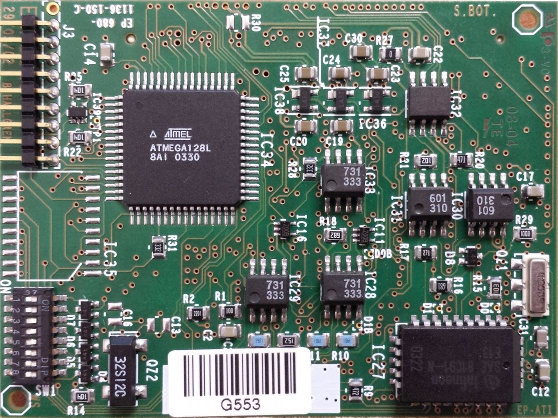
\includegraphics[height=75pt]{fig/elmb_photo}
  \end{changemargin}

  \setlength{\leftmargini}{2px}
  \begin{itemize}
    \item Features on-board programmable micro-processor.
  \end{itemize}
}

\frame{\frametitle{Low-Voltage monitoring}

}

\frame{\frametitle{Problems with present LV monitoring}

}

\frame{\frametitle{Addressing the issue}
  Inappropriate time scale. Compare LVPS time-scale with ELMB time-scale. Need faster digitization.
}

\frame{\frametitle{Use of trip transients for diagnostics}
  Show current from filter.\\
  Show voltage from output.
}

\frame{\frametitle{LVPS brick monitoring filter}

}

\frame{\frametitle{Use of trip transients for diagnostics}
  Show current from filter.\\
  Show voltage from filter.
}

\frame{\frametitle{10V brick transients}
  Show current from filter.\\
  Show voltage from filter. \\ .\\
  Explain that this is due to the filter.
}

\frame{\frametitle{Requirements for LVPS bricks}

}

\frame{\frametitle{Requirements for ELMB++}

}

\frame{\frametitle{Radiation tolerance requirements}

}

\frame{\frametitle{Requirements for DCS}

}

\frame{\frametitle{GBT-SCA alternative}
  \begin{changemargin}{-20px}{-20px}
    \centering
    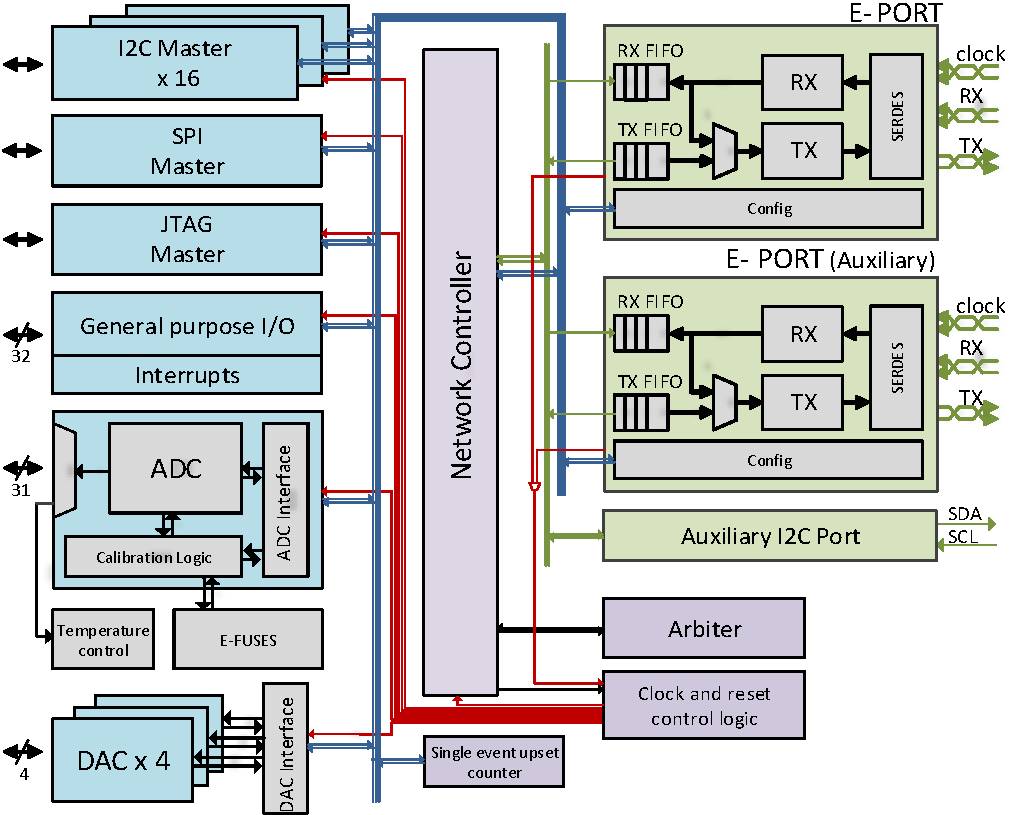
\includegraphics[height=140pt]{fig/gbt-sca_asic}
    \hspace{5px}
    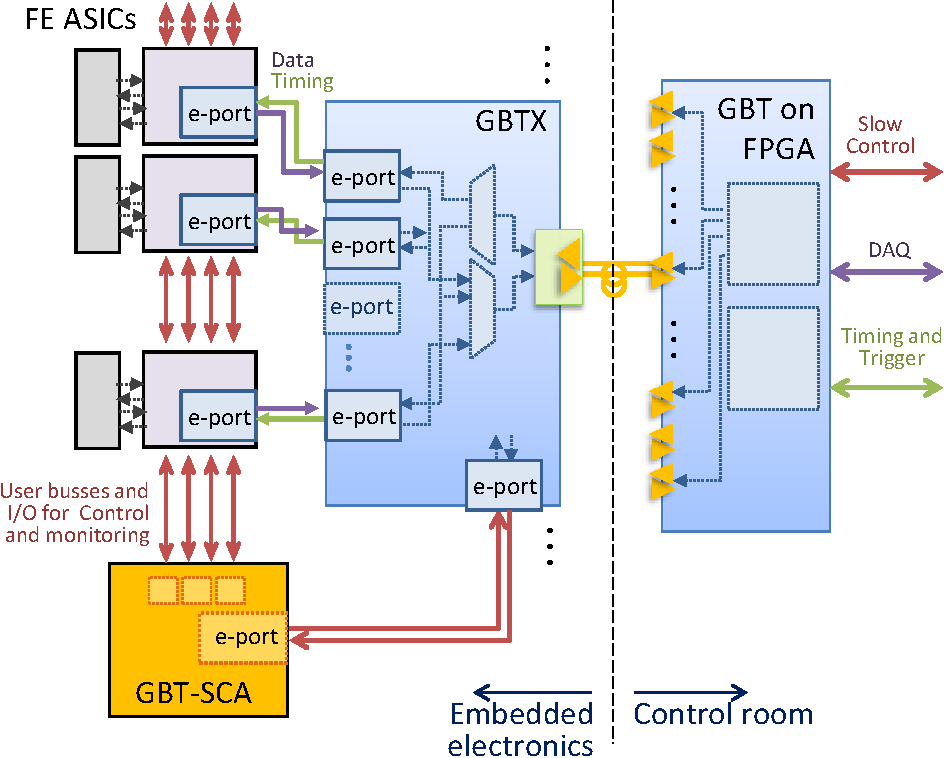
\includegraphics[height=140pt]{fig/gbt-sca_intercon}
  \end{changemargin}

  Text~\cite{cook05,henk11,henk03,giorgi12,sergei11,xadc,doc128,Usai:2026593,lvps_web,gary_lvps,gary_lvps_cds,hruska_brick,elmb_wiki,ATL-DAQ-2003-053,1748-0221-10-03-C03034,GBT-SCA-Manual6,GBT-SCA-Manual7}
}

\frame{\frametitle{Acknowledgements}
This material is based upon work at the Argonne National Laboratory supported by the U.S. Department of Energy, Office of Science,
Office of Workforce Development for Teachers and Scientists, Office of Science Graduate Student Research
(SCGSR) program. The SCGSR program is administered by the Oak Ridge Institute for Science and Education for
the DOE under contract number DE-AC05-06OR23100.
}

% BIBLIOGRAPHY
\begin{frame}[allowframebreaks]{Bibliography}% in case more than 1 slide needed
  \renewcommand*{\bibfont}{\tiny}
  \printbibliography
\end{frame}

\end{document}
